\documentclass[11pt]{article}

\usepackage[letterpaper,margin=1in]{geometry}
\usepackage[T1]{fontenc}
\usepackage[utf8]{inputenc}
\usepackage{textcomp}
\usepackage{lmodern}
\usepackage{amsmath,amssymb}
\usepackage{graphicx}
\usepackage{booktabs,longtable,array,calc}
\usepackage{caption}
\usepackage{hyperref}

\hypersetup{hidelinks}
\setcounter{secnumdepth}{2}
\setlength{\parindent}{0pt}
\setlength{\parskip}{0.6em}
\newcounter{none}
\providecommand{\tightlist}{\setlength{\itemsep}{0pt}\setlength{\parskip}{0pt}}

\title{Prospective Remeasurement Alerts for Suspicious Pediatric Growth Measurements in Electronic Health Records}
\author{[Author names and affiliations]}
\date{}

\begin{document}

\maketitle
\noindent\emph{[Corresponding author contact information]}

\noindent\textbf{Keywords:} pediatric growth, anthropometry, electronic health records, measurement error, remeasurement, longitudinal data quality, clinical decision support

\section*{Abstract}

\textbf{Objective.} To develop and preclinically evaluate a real-time electronic health record (EHR) alert for pediatric height measurements that may warrant immediate remeasurement while the child is still present.

\textbf{Materials and Methods.} We built a multi-detector, confidence-fused pipeline that uses only prior unflagged patient history at the time of height entry and returns a tunable remeasurement-alert score (default threshold 0.60). Performance was evaluated in streaming mode on six published Monte Carlo simulated-error benchmarks (Harrall et al.; 600 patients, 17,705 visits; 2,378 injected simulated errors), against streaming reimplementations of the Daymont and Harrall algorithms and the fixed 10\% prior-height-change rule used in EPIC. Operational burden was estimated in a de-identified outpatient pediatric EHR extract from the Pediatric Physicians' Organization at Children's (PPOC; 250,588 patients, 6,494,473 visits).

\textbf{Results.} At the default threshold, the pipeline detected 2,090 of 2,378 injected simulated errors and generated 669 false alerts among 15,327 non-injected visits (sensitivity 0.88, specificity 0.96), compared with streaming Harrall (0.71 / 0.95), streaming Daymont (0.82 / 0.99), and the EPIC rule (0.76 / 0.33). At threshold 0.70, simulated sensitivity remained 0.88 and specificity increased to 0.97 (2,078 true positives; 461 false positives). In the PPOC extract, the EPIC rule would have generated 1,764,100 alerts (27.2\% of visits). The pipeline's estimated alert burden was threshold dependent: 1,597,134 alerts (24.6\%) at the default threshold, 1,508,472 (23.2\%) at threshold 0.70, and 661,432 (10.2\%) at threshold 0.90.

\textbf{Conclusion.} In simulated streaming evaluation, a trajectory-aware remeasurement-alert pipeline achieved higher sensitivity than streaming comparator implementations and the EPIC rule, with lower specificity than Daymont. Real-world EHR analysis showed tunable alert volume rather than deployed predictive value. These findings support prospective clinical validation of remeasurement alerts as a practical strategy for obtaining contemporaneous reference measurements, but do not establish workflow impact or clinical utility.

\section{Background}\label{background}

A central obstacle in pediatric growth-data quality research is that the reference value for a clinical measurement is usually unavailable once the value has been saved to the electronic health record. A recorded height of 112 cm for a seven-year-old may reflect a genuine measurement, a transcription error, a unit confusion, or a carry-forward duplication of a prior visit's value --- and these possibilities cannot be reliably distinguished from the longitudinal record alone, even by trained clinicians with full access to the child's history. This limitation is not primarily an algorithmic shortcoming; it reflects the limited reference information available in retrospective EHR data. As Daymont noted, the same record contains both plausible outliers (true extreme values that look like errors) and implausible inliers (erroneous values that look ordinary against the population distribution but are wrong for the individual child) [7], and retrospective procedures have limited ability to separate these categories without an external reference measurement.

A substantial and sophisticated literature has developed retrospective cleaning algorithms that, given a child's full longitudinal record, attempt to declare each historical measurement plausible or implausible [1,2,6,9,10,11]. These algorithms are evaluated on either Monte Carlo simulated data with known injected errors [9] or human consensus labels whose inter-rater agreement is substantially below 1.0 [1] --- not because the field has been methodologically incautious, but because no better evidence base exists. The most widely adopted algorithm, Daymont's growthcleanr [1], has been validated against physician judgment and applied to large multisite consortia [4]; more recent approaches by Shi et al. [10], Phan et al. [6], and Harrall et al. [9] have introduced robust regression, peak-removal, and semi-parametric trajectory smoothing. All of these advances operate within the same evidentiary constraint.

Real-time clinical decision support in this domain is comparatively underdeveloped. The widely used EPIC EHR system alerts clinicians when a newly entered height differs from the immediately preceding visit by more than 10\%, and the clinician can either save or correct the value. As we show below, this rule has poor specificity --- it flags an enormous fraction of plausible growth --- and its anchoring to a single prior point makes it vulnerable to error propagation when the prior point was itself wrong. To our knowledge, trajectory-aware real-time height alerts are not currently standard commercial EHR functionality.

This paper proposes a prospective task formulation that addresses a practical limitation of retrospective labels. At the moment a new height is entered, while the child is still in the clinic, the original uncertainty can often still be reduced: a suspicious measurement can be repeated, and the clinician and patient are present to act on the result. We therefore reframe the task not as "is this historical measurement an error?" --- a question that retrospective records often cannot answer definitively --- but as "is this new measurement suspicious enough that we should remeasure it right now?" This shift does not prove error status after the fact, but it creates an opportunity to obtain a contemporaneous reference measurement while the ambiguity can still be acted on.

The central claim is therefore deliberately narrow. Retrospective labels remain useful but limited; prospective remeasurement offers a practical route to recoverable reference measurements; and the present study is a preclinical evaluation of streaming alert performance plus a retrospective analysis of operational alert burden. The operational consequences are also asymmetric in a clinically important way: a missed alert leaves the EHR in the same state it would otherwise be in, while a false alert costs a thirty-second remeasurement.

\section{Methods}\label{methods}

\subsection{Conceptual framing}\label{conceptual-framing}

The pipeline runs at the moment a new height is entered, while the child is still in the clinic. Every detector sees only the new measurement and the child's prior history --- no future points, in contrast to retrospective cleaning algorithms [1,9].

For each entered measurement the pipeline outputs a continuous error confidence in [0, 1] and a categorical label: error (population BIV or exact carry-forward duplicate), remeasure (fused confidence \(\ge\) alert threshold), or no alert. The clinician decides what to do with an alert --- remeasure or keep --- and the saved value is their choice.

For evaluation, we adopt one simplifying assumption: every alerted point is removed from the history available to subsequent points, equivalent to assuming each alert is acted on and resolved (either remeasured to truth or discarded). The same convention is applied to every comparator.

\subsection{Pipeline overview}\label{pipeline-overview}

The pipeline applies two hard rules and five soft detectors in sequence. The hard rules immediately raise an ``error'' alert if triggered. Otherwise, the five soft detectors are evaluated, each producing a confidence in [0, 1], and the five confidences are fused with a weighted noisy-OR rule [14] into a single error confidence. A ``remeasure'' alert is issued when the fused confidence clears the configured threshold.

\subsection{Hard rules}\label{hard-rules}

\textbf{Population BIV check.} Each new height is converted to a sex- and age-specific z-score using WHO Child Growth Standards for ages \(\le\) 1856 days [12] and CDC growth charts for ages \(>\) 1856 days [13]. For ages in the WHO range an absolute HAZ \(\ge\) 6 raises an error. In the CDC range the modified HAZ recommended by the CDC for extreme-value detection is used, with the CDC-recommended cutoffs of mod\_HAZ \(<\) -5 or mod\_HAZ \(>\) 4 [13].

\textbf{Carry-forward duplicate check.} A new height that matches the immediately previous observed height to within \(1 \times 10^{-6}\) cm raises an error. Exact equality between consecutive heights is essentially never the result of two independent measurements and is one of the most common error modes in EHR growth data --- Lin et al. report that carry-forward measurements were the most common error mode flagged in the PCORnet pediatric cohort, accounting for the majority of flagged pediatric heights [4]. Note that this check compares against the most recent \emph{observed} prior point, not the most recent \emph{un-flagged} point, so that a prior error followed by a carry-forward replication of that prior error is still caught.

\subsection{Soft detectors}\label{soft-detectors}

If the hard rules do not fire, the pipeline evaluates the following five detectors. All of them depend only on the new point and the patient's prior un-flagged history.

\textbf{Velocity (adjacent).} The short-interval velocity is computed as the change in height between the new point and the immediately preceding visit, divided by the age difference. Velocity is converted to an age- and sex-specific z-score against velocity reference distributions derived by numerical differentiation of the WHO and CDC LMS tables [12,13]. Adjacent velocity is the detector most sensitive to single-point errors: an isolated erroneous spike inflates the velocity both going in and coming out, so the adjacent-velocity z-score after the error is large in magnitude. Its threshold is \textbar z\textbar{} \(>\) 5.

\textbf{Velocity (adjusted).} The same velocity z-score, but computed against the most recent prior visit whose interval meets an age-specific minimum (90 days for ages 0--12 months, 180 days for ages 1--2 years, 335 days for ages 2--12 years, 180 days for ages 13--18 years, reflecting the shortest interval over which measurement noise is small relative to true growth). The adjusted velocity catches sustained shifts but, importantly, \emph{dilutes} a single-point error toward the population mean when the interval used is long.

\textbf{HAZ change.} The absolute change in HAZ between the new point and the immediately previous visit is compared to a dynamic, age- and interval-dependent plausibility threshold. This threshold is wider for younger children and longer intervals (during which legitimate channel-crossing growth shifts are larger) and narrower for older children and shorter intervals.

\textbf{Streaming LOWESS trajectory residual.} A robust LOWESS curve [15,16] is fit to the HAZ values in the patient's prior history (minimum five points) and extrapolated forward to the age of the new point. The residual --- new HAZ minus predicted HAZ --- is converted to a robust z by dividing by a residual scale, and the detector fires when \textbar z\textbar{} \(>\) 3.

The residual scale is estimated from self-free k-nearest-neighbor-median residuals: each history point is compared to the median HAZ of its five nearest-in-age neighbors (excluding itself), and the scale is 1.4826 \(\times\) MAD of those residuals [17]. The scale is then inflated by a \(\sqrt{1 + \mathrm{gap}/\tau}\) factor with \(\tau\) = 730 days when the new point lies well beyond the last history point, reflecting the fact that HAZ trajectories can legitimately drift over multi-year gaps even in healthy children.

\textbf{Soft HAZ magnitude.} A check on the magnitude of the new HAZ alone, threshold \textbar HAZ\textbar{} \(>\) 3, with a deliberately weak weight and a slow confidence ramp. We include this as a ``weak prior'' --- large HAZ values are more often than not real (Freedman et al. [8] cautioned exactly against treating extreme HAZ as automatic evidence of error) but are weakly informative when several other detectors also fire.

\subsection{Per-detector confidence mapping}\label{per-detector-confidence-mapping}

A detector that has not crossed its threshold contributes no evidence. Above the threshold, the per-detector confidence ramps smoothly toward 1 as a sigmoid of the \emph{exceedance ratio} r = \textbar metric\textbar{} / threshold:

\[c(r) = \left\{ \begin{aligned}
0,\ \  & r \leq 1 \\
\frac{1}{1 + \exp[-k(r - r_{\mathrm{mid}})]},\ \  & r > 1
\end{aligned} \right.\ \]

with k = 3.0 and a detector-specific \(r_{\mathrm{mid}}\). The exceedance form (rather than a sigmoid of the raw deviation) makes the curve scale-invariant across detectors with very different units (velocity z, HAZ, HAZ-change, trajectory z). The \(r_{\mathrm{mid}}\) parameter controls how far past the threshold a detector must reach before it contributes meaningful evidence: \(r_{\mathrm{mid}}\) = 1 would make a just-crossed threshold already score 0.5; we use \(r_{\mathrm{mid}}\) = 1.8 for the velocity and HAZ-change detectors and \(r_{\mathrm{mid}}\) = 2.0 for the soft-HAZ and trajectory detectors.

\subsection{Noisy-OR fusion}\label{noisy-or-fusion}

Per-detector confidences are pooled by weighted noisy-OR [14], the standard probabilistic combination rule for independent evidence:

\[C_{ensemble} = 1 - \prod_{i}^{}\left( 1 - w_{i} \cdot c_{i} \right)\]

with detector weights chosen to reflect each detector's expected reliability (adjacent velocity 0.85, adjusted velocity 0.90, HAZ change 0.90, trajectory 0.85, soft HAZ 0.45). This generalizes a ``k-of-N voting'' rule smoothly: any single detector with a high confidence can drive \(C_{\mathrm{ensemble}}\) high, multiple weak detectors can also accumulate to a high \(C_{\mathrm{ensemble}}\), and a detector that did not cross its threshold contributes nothing.

A ``remeasure'' alert is raised when \(C_{\mathrm{ensemble}}\) \(\ge\) \(\tau\), where \(\tau\) is a tunable threshold (default 0.60). The threshold sweep in Section~3.2 characterizes its tradeoff.

\subsection{Streaming application to retrospective benchmarks}\label{streaming-application-to-retrospective-benchmarks}

To evaluate the alert pipeline on retrospective benchmark data, we apply it in \emph{streaming} mode. For each patient, measurements are sorted in chronological order. The algorithm walks forward through the visits; for each visit, the history available to the detectors is the set of all prior un-flagged measurements for that patient. Once a measurement is flagged (as either ``error'' or ``remeasure''), it is removed from the history that subsequent points are judged against.

This streaming protocol is the faithful simulation of the live-EHR deployment: at the moment of entry, the algorithm has the patient's curated prior history and is asked whether the new point should trigger an alert. We use the same protocol below to evaluate the Daymont and Harrall algorithms for fair comparison.

\subsection{Evaluation data}\label{evaluation-data}

We use the Monte Carlo simulated-error datasets released with the Harrall paper [9], which were generated by:

\begin{enumerate}
\def\labelenumi{\arabic{enumi}.}
\item
  Simulating clean longitudinal height trajectories for 100 children each, from a Preece--Baines [18] parametric growth model with three parameter sets corresponding to ``low,'' ``medium,'' and ``high'' populations (positioned at the 5th--25th, 25th--75th, and 75th--95th CDC percentile bands, respectively).
\item
  Generating 100 visits per child with mean and variance of visit spacing matched to the EPOCH cohort [19].
\item
  Injecting three classes of errors at known positions and magnitudes:
\end{enumerate}

\begin{itemize}
\item
  \textbf{Cups} --- abrupt downward height excursions that recover at the next visit (e.g., a transcription mistake);
\item
  \textbf{Caps} --- abrupt upward height excursions that recover at the next visit;
\item
  \textbf{Repeats} --- exact duplicates of the previous visit's height value, simulating EHR carry-forward auto-population.
\end{itemize}

\begin{enumerate}
\def\labelenumi{\arabic{enumi}.}
\setcounter{enumi}{3}
\item
  Varying the error rate across two levels labeled ``dirt2'' (matching the empirical error proportions estimated from the EPOCH cohort) and ``dirt3'' (double the empirical error rate).
\end{enumerate}

The released benchmark thus consists of six labeled datasets --- pop\{1,2,3\}\_dirt\{2,3\} --- with bad\_ht = True marking every injected error. Table 1 summarizes these benchmarks; total visits range from 2,818 to 3,022 per dataset, and the simulated error prevalence ranges from 10.4\% to 16.2\%.

\textbf{Table 1.} Composition of the six Harrall simulated-error benchmarks.

{\def\LTcaptype{none} % do not increment counter
\begin{longtable}[]{@{}
  >{\raggedright\arraybackslash}p{(\linewidth - 8\tabcolsep) * \real{0.1824}}
  >{\raggedleft\arraybackslash}p{(\linewidth - 8\tabcolsep) * \real{0.1395}}
  >{\raggedleft\arraybackslash}p{(\linewidth - 8\tabcolsep) * \real{0.1502}}
  >{\raggedleft\arraybackslash}p{(\linewidth - 8\tabcolsep) * \real{0.2575}}
  >{\raggedleft\arraybackslash}p{(\linewidth - 8\tabcolsep) * \real{0.2575}}@{}}
\toprule\noalign{}
\begin{minipage}[b]{\linewidth}\raggedright
\textbf{Dataset}
\end{minipage} & \begin{minipage}[b]{\linewidth}\raggedleft
\textbf{Patients}
\end{minipage} & \begin{minipage}[b]{\linewidth}\raggedleft
\textbf{Visits}
\end{minipage} & \begin{minipage}[b]{\linewidth}\raggedleft
\textbf{Injected errors}
\end{minipage} & \begin{minipage}[b]{\linewidth}\raggedleft
\textbf{Error prevalence}
\end{minipage} \\
\midrule\noalign{}
\endhead
\bottomrule\noalign{}
\endlastfoot
pop1\_dirt2 & 100 & 2,932 & 362 & 12.3\% \\
pop1\_dirt3 & 100 & 2,987 & 475 & 15.9\% \\
pop2\_dirt2 & 100 & 2,960 & 308 & 10.4\% \\
pop2\_dirt3 & 100 & 2,818 & 457 & 16.2\% \\
pop3\_dirt2 & 100 & 2,986 & 324 & 10.9\% \\
pop3\_dirt3 & 100 & 3,022 & 452 & 15.0\% \\
\textbf{Total} & \textbf{600} & \textbf{17,705} & \textbf{2,378} & \textbf{13.4\%} \\
\end{longtable}
}

\subsection{Comparators}\label{comparators}

We compare to three streaming baselines:

\begin{itemize}
\item
  \textbf{Streaming Daymont.} The Daymont weighted-moving-average algorithm [1] (growthcleanr) applied to each successive truncation of a patient's history, so that the decision for visit \emph{t} uses only history up to visit \emph{t} - 1.
\item
  \textbf{Streaming Harrall.} The Harrall trajectory-cleaning algorithm [9] applied to each successive history truncation.
\item
  \textbf{EPIC 10\% rule.} A new measurement is flagged when its height differs from the most recent un-flagged previous height by more than 10\%, mimicking the rule used in the EPIC EHR. Flagged points are removed from history for subsequent checks.
\end{itemize}

The Daymont and Harrall algorithms were not designed for prospective use; we include them for completeness so that we can quantify how much each loses by removing bidirectional context.

\section{Results}\label{results}

\subsection{Performance at the default threshold}\label{performance-at-the-default-threshold}

Table 2 reports per-dataset sensitivity and specificity for all four algorithms at the default alert threshold (0.60 for our pipeline, 0.10 for EPIC).

\textbf{Table 2.} Sensitivity / specificity by dataset and method, streaming mode.

{\def\LTcaptype{none} % do not increment counter
\begin{longtable}[]{@{}
  >{\raggedright\arraybackslash}p{(\linewidth - 8\tabcolsep) * \real{0.1609}}
  >{\raggedleft\arraybackslash}p{(\linewidth - 8\tabcolsep) * \real{0.2039}}
  >{\raggedleft\arraybackslash}p{(\linewidth - 8\tabcolsep) * \real{0.2039}}
  >{\raggedleft\arraybackslash}p{(\linewidth - 8\tabcolsep) * \real{0.1824}}
  >{\raggedleft\arraybackslash}p{(\linewidth - 8\tabcolsep) * \real{0.2361}}@{}}
\toprule\noalign{}
\begin{minipage}[b]{\linewidth}\raggedright
\textbf{Dataset}
\end{minipage} & \begin{minipage}[b]{\linewidth}\raggedleft
\textbf{Harrall (streaming)}
\end{minipage} & \begin{minipage}[b]{\linewidth}\raggedleft
\textbf{Daymont (streaming)}
\end{minipage} & \begin{minipage}[b]{\linewidth}\raggedleft
\textbf{EPIC 10\%}
\end{minipage} & \begin{minipage}[b]{\linewidth}\raggedleft
\textbf{This work}
\end{minipage} \\
\midrule\noalign{}
\endhead
\bottomrule\noalign{}
\endlastfoot
pop1\_dirt2 & 0.68 / 0.94 & 0.79 / 0.99 & 0.73 / 0.39 & \textbf{0.87 / 0.97} \\
pop1\_dirt3 & 0.75 / 0.96 & 0.85 / 1.00 & 0.77 / 0.28 & \textbf{0.91 / 0.96} \\
pop2\_dirt2 & 0.67 / 0.96 & 0.80 / 0.99 & 0.77 / 0.30 & \textbf{0.87 / 0.94} \\
pop2\_dirt3 & 0.70 / 0.91 & 0.82 / 0.98 & 0.81 / 0.28 & \textbf{0.86 / 0.93} \\
pop3\_dirt2 & 0.72 / 0.97 & 0.80 / 0.99 & 0.73 / 0.36 & \textbf{0.87 / 0.98} \\
pop3\_dirt3 & 0.72 / 0.95 & 0.83 / 0.99 & 0.74 / 0.36 & \textbf{0.89 / 0.96} \\
\textbf{Pooled} & \textbf{0.71 / 0.95} & \textbf{0.82 / 0.99} & \textbf{0.76 / 0.33} & \textbf{0.88 / 0.96} \\
\end{longtable}
}

The EPIC 10\% rule has by far the lowest specificity (0.33 pooled), reflecting the well-known overflagging of normal pediatric growth by a fixed 10\% rule --- adolescent growth spurts and early-childhood velocity routinely produce \(>\) 10\% height changes per visit. The Harrall algorithm loses substantial sensitivity in streaming mode (0.71 pooled, compared with \(>\) 0.99 reported in its retrospective evaluation [9]); the design of its peak-removal step relies on the existence of a downward ``cup'' \emph{after} a flagged ``cap,'' and that future point is unavailable in streaming use. The Daymont algorithm's weighted moving average uses inverse-distance weighting that gives current and recent points more weight, which translates better to streaming use and degrades less (pooled sensitivity 0.82, specificity 0.99). Daymont also retains the highest specificity of all four methods, exceeding our pipeline's 0.96 by 3 percentage points. Our pipeline achieves the highest pooled sensitivity (0.88) of the four, with specificity (0.96) competitive with the retrospective-style baselines and far above EPIC.

\subsection{Threshold sensitivity sweep}\label{threshold-sensitivity-sweep}

To characterize the alert threshold's tradeoff, we re-ran the streaming pipeline on all six datasets at remeasure-confidence thresholds 0.30 through 0.90 in increments of 0.10. Because a flagged point is removed from history for subsequent decisions, each threshold is a full re-run, not a post-hoc re-thresholding of cached scores.

\textbf{Table 3.} Pooled sensitivity / specificity across all six datasets vs. alert threshold.

{\def\LTcaptype{none} % do not increment counter
\begin{longtable}[]{@{}
  >{\raggedleft\arraybackslash}p{(\linewidth - 10\tabcolsep) * \real{0.1719}}
  >{\raggedleft\arraybackslash}p{(\linewidth - 10\tabcolsep) * \real{0.1719}}
  >{\raggedleft\arraybackslash}p{(\linewidth - 10\tabcolsep) * \real{0.1396}}
  >{\raggedleft\arraybackslash}p{(\linewidth - 10\tabcolsep) * \real{0.1396}}
  >{\raggedleft\arraybackslash}p{(\linewidth - 10\tabcolsep) * \real{0.1826}}
  >{\raggedleft\arraybackslash}p{(\linewidth - 10\tabcolsep) * \real{0.1826}}@{}}
\toprule\noalign{}
\begin{minipage}[b]{\linewidth}\raggedleft
\textbf{Threshold}
\end{minipage} & \begin{minipage}[b]{\linewidth}\raggedleft
\textbf{Alerted}
\end{minipage} & \begin{minipage}[b]{\linewidth}\raggedleft
\textbf{TP}
\end{minipage} & \begin{minipage}[b]{\linewidth}\raggedleft
\textbf{FP}
\end{minipage} & \begin{minipage}[b]{\linewidth}\raggedleft
\textbf{Sensitivity}
\end{minipage} & \begin{minipage}[b]{\linewidth}\raggedleft
\textbf{Specificity}
\end{minipage} \\
\midrule\noalign{}
\endhead
\bottomrule\noalign{}
\endlastfoot
0.30 & 3,727 & 2,115 & 1,612 & 0.89 & 0.89 \\
0.40 & 3,261 & 2,106 & 1,155 & 0.89 & 0.92 \\
0.50 & 3,105 & 2,098 & 917 & 0.88 & 0.94 \\
\textbf{0.60} & \textbf{2,759} & \textbf{2,090} & \textbf{669} & \textbf{0.88} & \textbf{0.96} \\
0.70 & 2,539 & 2,078 & 461 & 0.88 & 0.97 \\
0.80 & 2,410 & 2,060 & 350 & 0.87 & 0.98 \\
0.90 & 2,131 & 1,894 & 237 & 0.80 & 0.98 \\
\end{longtable}
}

The tradeoff is asymmetric. Between thresholds 0.30 and 0.80, sensitivity declines only modestly (0.89 \(\to\) 0.87); the false-positive count falls almost five-fold (1,612 \(\to\) 350) for the cost of 55 true positives (2.6\% relative loss in TP). Only beyond threshold 0.80 does sensitivity drop steeply. The operational implication is that a clinic with low tolerance for false alarms could move the threshold up to 0.80 with little loss of simulated-error capture, and only at the most conservative end (\(\ge\) 0.90) does the algorithm begin to miss meaningfully more injected errors.

\begin{figure}[htbp]
\centering
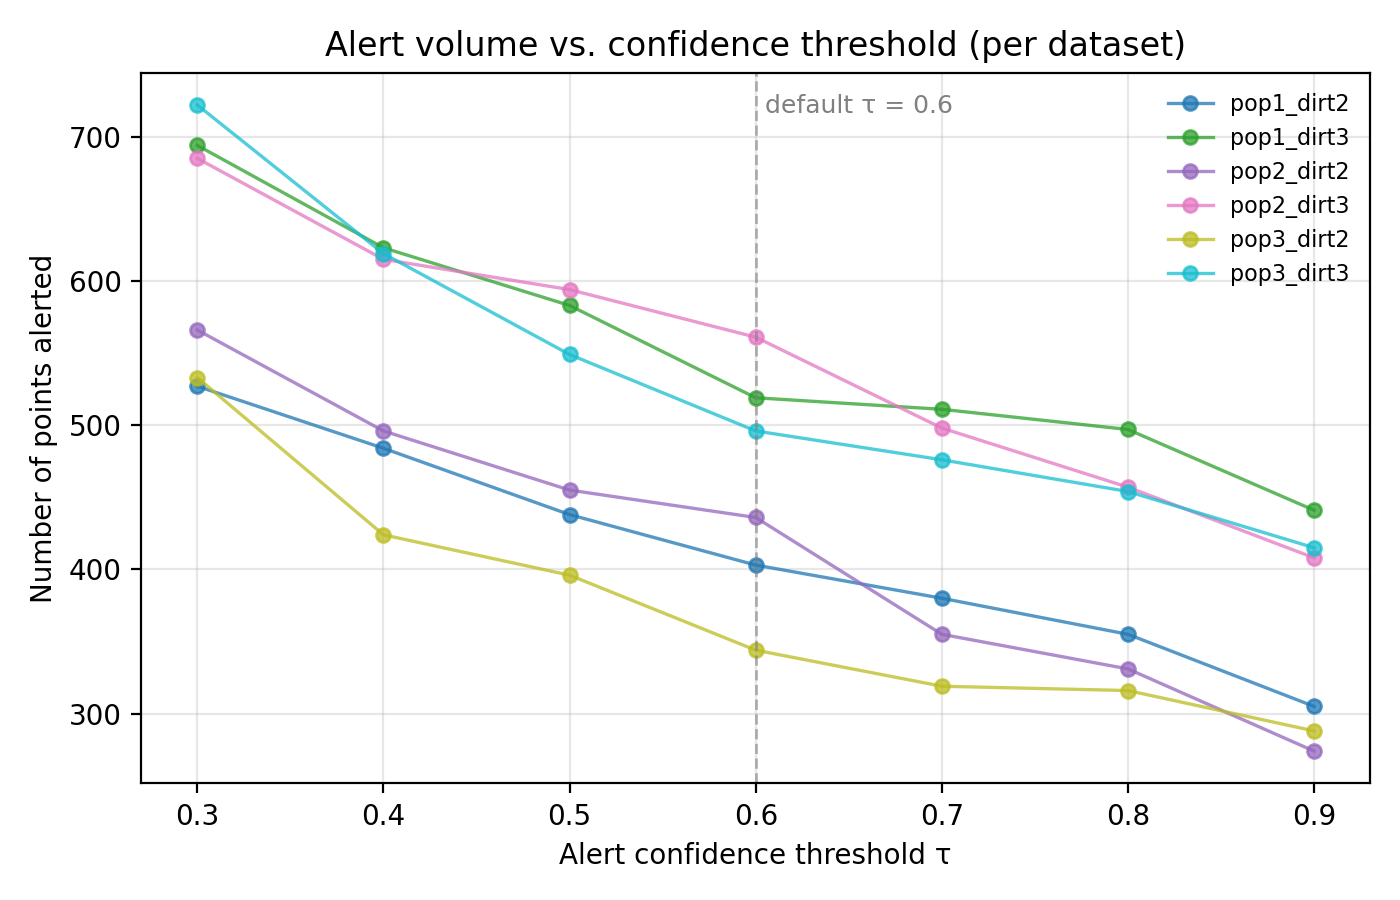
\includegraphics[width=6.5in,height=4.17847in]{figures/fig1_threshold_alerts.png}
\caption{Number of points alerted as a function of the confidence threshold \(\tau\), shown separately for each of the six simulated-error datasets. The dashed vertical line marks the default threshold (\(\tau\) = 0.60).}
\label{fig:1}
\end{figure}

\begin{figure}[htbp]
\centering
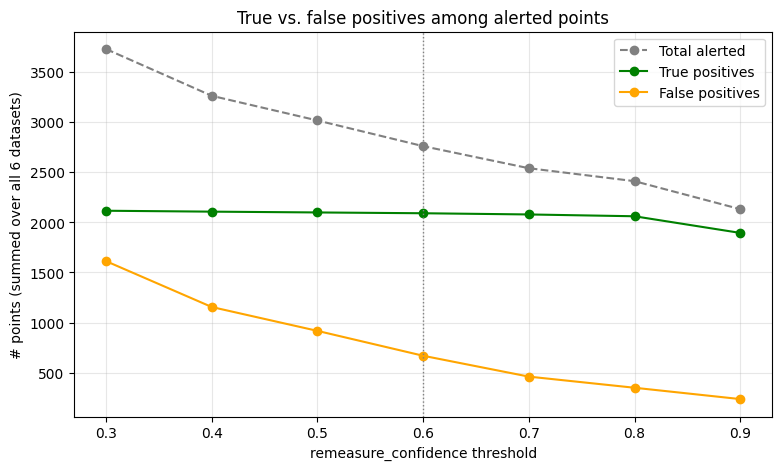
\includegraphics[width=6.5in,height=3.90903in]{figures/fig2_alerts_by_outcome.png}
\caption{Alerted points pooled across all six datasets, decomposed as a function of the confidence threshold \(\tau\). The dashed gray line is the total number of points alerted; the green line is the subset that are true positives (correctly flagged simulated errors); the orange line is the subset that are false positives (clean points incorrectly flagged).}
\label{fig:2}
\end{figure}

\subsection{Operational alert burden on a real-world EHR cohort}\label{operational-alert-burden-on-a-real-world-ehr-cohort}

\textbf{Dataset.} We used a de-identified longitudinal EHR extract from the Pediatric Physicians' Organization at Children's (PPOC), a primary-care network affiliated with Boston Children's Hospital. The cohort comprises 250,588 unique pediatric patients aged 0--18 years, with 6,494,473 clinical visits (\(\approx\) 72.8\% routine office visits) recorded across the network. Each visit row carries patient demographics (sex, ethnicity, race), encounter type, anthropometrics (height, weight, BMI and derived percentiles), and up to 33 ICD-10 encounter diagnoses; the broader extract also includes 17.2 M laboratory result components, 3.8 M medication records, 1.7 M problem-list entries, and 349,827 specialty referrals, all linked by \texttt{patient\_id} and \texttt{visit\_id}. Dates are de-identified as \texttt{age\_in\_days}. For the present analysis we used only the height column from the visits table. Unlike the Harrall simulator, no ground-truth error labels are available, so this analysis reports alert volume --- the count and share of measurements that would trigger an alert --- rather than sensitivity or specificity.

\textbf{Analysis.} To characterize the operational burden the two approaches would impose in live clinical use, we ran both the EPIC 10\% rule and our pipeline (in streaming mode, across the same threshold sweep used in Section~3.2) on every height measurement in the cohort, removing flagged points from each patient's running history as in the simulated-benchmark protocol.

\begin{figure}[htbp]
\centering
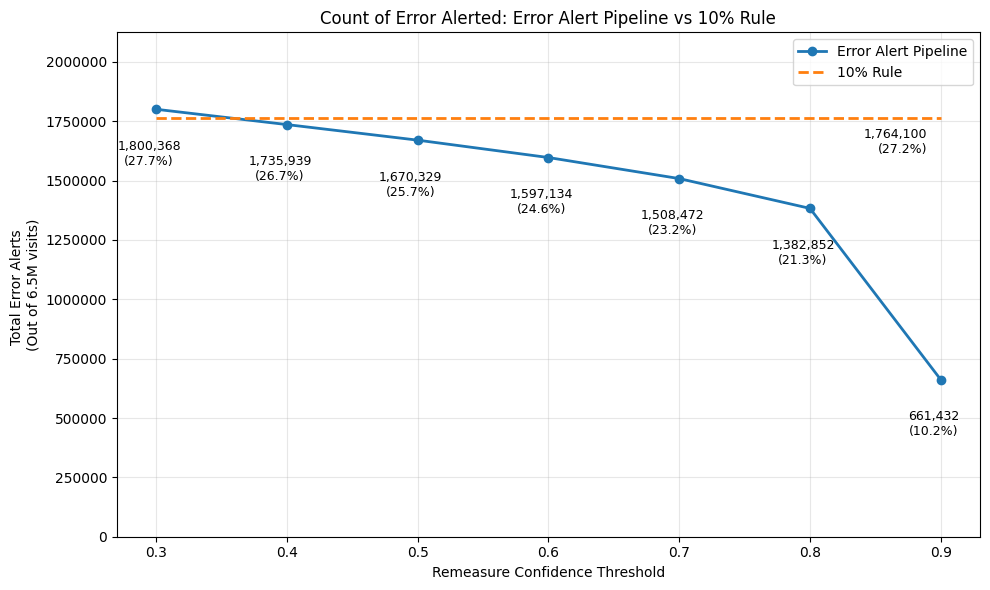
\includegraphics[width=6.5in,height=3.87083in]{figures/fig3_ppoc_alert_burden.png}
\caption{Total number of height measurements that would trigger an alert in the PPOC cohort (\(\approx\) 6.5 M visits) under the EPIC 10\% rule (orange dashed) and under the error alert pipeline at remeasure-confidence thresholds from 0.30 to 0.90 (solid blue). Annotations report absolute counts and the percentage of the full cohort.}
\label{fig:3}
\end{figure}

The EPIC 10\% rule alerts on roughly 1.76 million measurements (\(\approx\) 27\% of all visits). Across the evaluated thresholds, the pipeline would have generated far fewer alerts in this retrospective EHR extract, and the threshold sweep quantifies the tradeoff between simulated-error sensitivity and expected remeasurement burden. These results suggest that trajectory-aware alerting could reduce alert volume relative to the EPIC rule, but prospective deployment is needed to measure adherence, PPV, false negatives, and workflow impact in practice.

\section{Discussion}\label{discussion}

\subsection{Central claim and scope}\label{central-claim-and-scope}

The main contribution of this paper is not a final adjudication method for all historical growth measurements. It is a prospective problem formulation for pediatric growth-data quality. Retrospective cleaning methods remain valuable, but they operate under an important evidentiary constraint: once a measurement has been saved, the original physical measurement cannot usually be repeated under the same clinical circumstances. Simulated benchmarks and human consensus labels are therefore useful but incomplete evaluation tools for methods intended to identify real clinical measurement errors.

Prospective alerting changes the available evidence. If an alert fires while the child is still present, immediate remeasurement can provide a contemporaneous reference measurement and can directly test whether the alert identified a value that would change with repeat measurement. This does not eliminate all uncertainty, because remeasurement itself has error and workflow adherence may vary, but it provides a practical path to stronger external validation than retrospective record review alone.

The present evaluation supports only that bounded claim. The simulated benchmark is useful for comparing methods under controlled error assumptions, and the PPOC EHR analysis estimates the operational burden such alerts would create in real traffic. Together, these analyses test whether a prospective remeasurement strategy is technically and operationally plausible. They do not establish clinical superiority, predictive value in deployed use, or workflow acceptability. Section 4.4 outlines the prospective study required to establish those claims.

\subsection{Comparison to EPIC 10\% rule}\label{comparison-to-epic-10-rule}

The EPIC 10\% rule's low specificity in the Harrall simulated-error benchmark (0.33 pooled) reflects a mismatch between a fixed proportional threshold and pediatric growth physiology. Children grow at strongly age-dependent velocities, and 10\% per visit is easily exceeded by ordinary growth in infants (\(\approx\) 50\% per year), early adolescents during peak height velocity, and any child with intervisit gaps of more than a year. Our results suggest that even a small amount of trajectory awareness --- at minimum, age- and sex-adjusted velocity z-scores --- could substantially reduce alert burden in EHRs that currently use the 10\% rule, without sacrificing the simulated sensitivity to gross errors that motivated the rule in the first place.

\subsection{Limitations}\label{limitations}

The primary limitation of this evaluation follows directly from its scope: it is a preclinical streaming evaluation, not a deployed clinical validation study. Once a measurement has been saved, the original clinical measurement usually cannot be repeated under the same circumstances, so retrospective studies must rely on simulated errors, consensus labels, or other imperfect reference standards. This paper uses that same evidentiary base for benchmark comparison and adds a retrospective EHR analysis of alert burden. The prospective framing is valuable because it could collect contemporaneous repeat measurements when an alert fires, allowing future studies to estimate predictive value, adherence, and workflow impact directly in clinical use; sensitivity would require additional repeat measurement of a sample of unalerted visits, as outlined below.

\textbf{No weight evaluation.} This work covers only height; weight is more difficult because legitimate short-term decreases are common and would require different velocity and HAZ-change references. Extension to weight is a natural next step.

\textbf{Static thresholds and weights.} The detector weights and \(r_{\mathrm{mid}}\) parameters are hand-chosen based on simulator-tuning and clinical reasoning; they could in principle be learned from a labeled training set. We did not pursue this because the Harrall simulator's error distribution is itself synthetic and learning weights on it risks overfitting to assumptions that do not hold in real data.

\subsection{Future directions}\label{future-directions}

The arguments in Section~4.1 and Section~4.3 motivate a prospective in-clinic study in which the algorithm fires, the child is remeasured before they leave the room, and the original--remeasurement pair is recorded for evaluation. This design would estimate PPV, sensitivity, adherence, and workflow burden using contemporaneous repeat measurements rather than retrospective labels alone. We outline below a protocol intended to support a multi-site evaluation.

\textbf{Study design.} A prospective, multi-site observational deployment study in pediatric primary-care clinics with EHR-integrated growth charting (e.g., participating PPOC sites). The pipeline runs as a real-time decision support widget invoked at the moment a height is committed in the EHR. When the fused confidence exceeds the deploying clinic's threshold (default 0.60), the medical assistant or nurse who recorded the initial measurement is prompted, before the visit closes, to repeat the measurement using a standardized protocol. Both values, the time elapsed between them, the firing detectors, and the fused confidence are written to a study log; the EHR-saved value remains the clinician's choice and is also logged. Independent of alert firing, a random 1--2\% sample of unalerted measurements is also remeasured to estimate the false-negative rate.

\textbf{Primary endpoints.} (i) Positive predictive value (PPV) of the alert at the default threshold, with 95\% confidence interval; (ii) PPV as a function of the confidence threshold across the same sweep used in Section~3.2; (iii) sensitivity, estimated from the random-sample remeasurement arm.

\textbf{Clinician workflow and adherence.} The alert appears as a non-blocking modal immediately on save, with a one-line rationale derived from the firing detectors (e.g., "implausible velocity since previous visit; HAZ change above age-adjusted threshold"). The remeasurement step is logged whether or not it is performed; non-adherence is itself a primary descriptive outcome, since a CDS alert that is consistently dismissed is operationally a failed alert regardless of its statistical performance.

This protocol is, in our view, the appropriate next study. The simulated benchmarks in Section~3 establish that the algorithm is competitive in the regime where ground truth is artificially available; the PPOC analysis in Section~3.3 establishes that it produces a tractable alert burden in real EHR traffic; what remains is to establish, on real patients, that the alerts it does produce correspond to measurements a careful remeasurement would in fact change.

Two extensions are worth flagging beyond the prospective study above. First, extending the same pipeline to weight, with appropriate reference standards and an additional set of detectors that handle plausible short-term decreases. Second, exploring representation choices for downstream learning: whether large language models or other learned models perform better when growth data are presented as raw measurements, z-scores, percentiles, velocity features, or growth-chart images.

\section{Conclusion}\label{conclusion}

The central contribution of this paper is a prospective framing of the growth-data quality problem. Retrospective adjudication is constrained because the original clinical measurement usually cannot be repeated after the fact, leaving simulated errors and human consensus labels as imperfect but useful references. A prospective alert, by contrast, fires at the moment of entry, while the child and clinician are present and remeasurement is possible. This framing turns some uncertain retrospective judgments into actionable opportunities for repeat measurement and creates a path to recoverable reference measurements.

Within this bounded claim, the multi-detector confidence-fused pipeline presented here achieved pooled sensitivity 0.88 and specificity 0.96 on the Harrall Monte Carlo benchmark in streaming mode, with higher sensitivity than streaming Harrall and Daymont implementations, lower specificity than Daymont, and much higher specificity than the EPIC 10\% rule. In the PPOC EHR extract, the same thresholds would have produced far fewer alerts than the EPIC rule. These findings support prospective evaluation of trajectory-aware remeasurement alerts, but do not by themselves establish clinical effectiveness, workflow acceptability, or generalizability across EHR implementations.

\section*{References}\label{references}

\begin{enumerate}
\def\labelenumi{\arabic{enumi}.}
\item
  Daymont C, Ross ME, Localio AR, Fiks AG, Wasserman RC, Grundmeier RW. Automated identification of implausible values in growth data from pediatric electronic health records. \emph{J Am Med Inform Assoc.} 2017;24(6):1080--1087. doi:10.1093/jamia/ocx037.
\item
  Yang S, Hutcheon JA. Identifying outliers and implausible values in growth trajectory data. \emph{Ann Epidemiol.} 2016;26(1):77--80.e2. doi:10.1016/j.annepidem.2015.10.002.
\item
  Carsley S, Parkin PC, Tu K, et al. Reliability of routinely collected anthropometric measurements in primary care.~\emph{BMC Med Res Methodol}. 2019;19(1):84. Published 2019 Apr 24. doi:10.1186/s12874-019-0726-8.
\item
  Lin PD, Rifas-Shiman SL, Aris IM, Daley MF, Janicke DM, Heerman WJ, Chudnov DL, Freedman DS, Block JP. Cleaning of anthropometric data from PCORnet electronic health records using automated algorithms. \emph{JAMIA Open.} 2022;5(4):ooac089. doi:10.1093/jamiaopen/ooac089.
\item
  Ulijaszek SJ, Kerr DA. Anthropometric measurement error and the assessment of nutritional status. \emph{Br J Nutr.} 1999;82(3):165--177. doi:10.1017/S0007114599001348.
\item
  Phan HTT, Borca F, Cable D, Batchelor J, Davies JH, Ennis S. Automated data cleaning of paediatric anthropometric data from longitudinal electronic health records: protocol and application to a large patient cohort. \emph{Sci Rep.} 2020;10(1):10164. doi:10.1038/s41598-020-66925-7.
\item
  Daymont C. Plausible outliers and implausible inliers. \emph{Obesity (Silver Spring).} 2020;28(7):1174. doi:10.1002/oby.22865.
\item
  Freedman DS, Lawman HG, Skinner AC, McGuire LC, Allison DB, Ogden CL. Validity of the WHO cutoffs for biologically implausible values of weight, height, and BMI in children and adolescents in NHANES from 1999 through 2012. \emph{Am J Clin Nutr.} 2015;102(5):1000--1006. doi:10.3945/ajcn.115.115576.
\item
  Harrall KK, Bird SM, Muller KE, Vanderlinden LA, Payton ME, Bellatorre A, Dabelea D, Glueck DH. A better performing algorithm for identification of implausible growth data from longitudinal pediatric medical records. \emph{Sci Rep.} 2024;14(1):18276. doi:10.1038/s41598-024-69161-5.
\item
  Shi J, Korsiak J, Roth DE. New approach for the identification of implausible values and outliers in longitudinal childhood anthropometric data. \emph{Ann Epidemiol.} 2018;28(3):204--211.e3. doi:10.1016/j.annepidem.2018.01.007.
\item
  Thurber KA, Banks E, Banwell C. Approaches to maximising the accuracy of anthropometric data on children: review and empirical evaluation using the Australian Longitudinal Study of Indigenous Children. \emph{Public Health Res Pract.} 2014;25(1):e2511407. doi:10.17061/phrp2511407.
\item
  de Onis M, Garza C, Victora CG, Onyango AW, Frongillo EA, Martines J; WHO Multicentre Growth Reference Study Group. The WHO Multicentre Growth Reference Study: planning, study design, and methodology. \emph{Food Nutr Bull.} 2004;25(1 Suppl 1):S15--S26. doi:10.1177/15648265040251S104.
\item
  Kuczmarski RJ, Ogden CL, Guo SS, Grummer-Strawn LM, Flegal KM, Mei Z, Wei R, Curtin LR, Roche AF, Johnson CL. 2000 CDC growth charts for the United States: methods and development. \emph{Vital Health Stat 11.} 2002;(246):1--190.
\item
  Pearl J. \emph{Probabilistic Reasoning in Intelligent Systems: Networks of Plausible Inference.} San Mateo, CA: Morgan Kaufmann; 1988. ISBN 978-1558604797.
\item
  Cleveland WS. Robust locally weighted regression and smoothing scatterplots. \emph{J Am Stat Assoc.} 1979;74(368):829--836. doi:10.1080/01621459.1979.10481038.
\item
  Cleveland WS, Devlin SJ. Locally weighted regression: an approach to regression analysis by local fitting. \emph{J Am Stat Assoc.} 1988;83(403):596--610. doi:10.1080/01621459.1988.10478639.
\item
  Rousseeuw PJ, Croux C. Alternatives to the median absolute deviation. \emph{J Am Stat Assoc.} 1993;88(424):1273--1283. doi:10.1080/01621459.1993.10476408.
\item
  Preece MA, Baines MJ. A new family of mathematical models describing the human growth curve. \emph{Ann Hum Biol.} 1978;5(1):1--24. doi:10.1080/03014467800002601.
\item
  Crume TL, Ogden L, West NA, Vehik KS, Scherzinger A, Daniels S, McDuffie R, Bischoff K, Hamman RF, Norris JM, Dabelea D. Association of exposure to diabetes in utero with adiposity and fat distribution in a multiethnic population of youth: the Exploring Perinatal Outcomes among Children (EPOCH) Study. \emph{Diabetologia.} 2011;54(1):87--92. doi:10.1007/s00125-010-1925-3.
\end{enumerate}

\end{document}
